\documentclass[a4paper,12pt]{article}
\usepackage[hidelinks]{hyperref}
\usepackage{xcolor}
\usepackage{graphicx}
\usepackage{subfigure}
\usepackage{float}
\usepackage{amsmath}
\usepackage{algorithm}
\usepackage{listings}
\usepackage{xcolor}

\lstset{
    language=Python,
    basicstyle=\ttfamily\small,
    numbers=left,
    numberstyle=\tiny,
    stepnumber=1,
    backgroundcolor=\color{lightgray},
    frame=single,
    captionpos=b,
    breaklines=true,
    showstringspaces=false,
}

\lstset{
    language = Python,
    backgroundcolor = \color{yellow!10},    % 背景色:淡黄
    basicstyle = \small\ttfamily,           % 基本样式 + 小号字体
    rulesepcolor= \color{gray},             % 代码块边框颜色
    breaklines = true,                  % 代码过长则换行
    numbers = left,                     % 行号在左侧显示
    numberstyle = \small,               % 行号字体
    keywordstyle = \color{blue},            % 关键字颜色
    commentstyle =\color{green!100},        % 注释颜色
    stringstyle = \color{red!100},          % 字符串颜色
    frame = shadowbox,                  % 用(带影子效果)方框框住代码块
    showspaces = false,                 % 不显示空格
    columns = fixed,                    % 字间距固定 
    %escapeinside={<@}{@>}              % 特殊自定分隔符:<@可以自己加颜色@>
    morekeywords = {as},                % 自加新的关键字(必须前后都是空格)
    deletendkeywords = {compile}        % 删除内定关键字;删除错误标记的关键字用deletekeywords删!
}



\begin{document}
    \title{Linear and Convex Optimization: Project}
    \author{Yu Junjie}
    \date{\today}
    \maketitle

    \pagenumbering{roman}
    {\large\tableofcontents}
    \newpage
    \pagenumbering{arabic}

    \section{Obejective of the Experiment}
    \subsection{Representation of the Problem}
    \
    \newline
    \indent The goal of the project is to develop a program to solve the \textit{Water-filling} problem. And the \textit{Water-filling} problem can be represent as a convex optimization problem as below:
    \begin{align}
        \text{minimize} \hspace{1cm} &-\sum_{i = 1}^{n} \log (\alpha_i + x_i) \\
        \text{subject to}  \hspace{1cm} &x\succeq 0, \textbf{1}^T x = 1
    \end{align}
    where $\alpha_i > 0$. And use the KKT condition, we obtain the following relations:
    \begin{align}
        &x^* \succeq 0, \hspace{0.5cm}\textbf{1}^T x^* = 1 \\
        &x_i^*(\nu^* - 1/(\alpha_i + x_i^*)) = 0, \hspace{1.5cm}\text{where $i = 1,\dots,n$} \\
        &-1/(\alpha_i + x_i^*) - \lambda_i^*+\nu^* = 0, \hspace{1cm}\text{where $i = 1,\dots,n$}
    \end{align}
    
    After solving the equations that the KKT condition gives, we can finally change the \textit{Water-filling} problem to solve the equation that:
    \begin{align}
        x_i^* = \max(0, 1/\nu^* - \alpha_i)
    \end{align} 
    where $\nu^*$ is determined by solving: 
    \begin{align}
        \sum_{i = 1}^{n} x_i^* = 1 
    \end{align}
    The value of $\nu^*$ is found by adjusting it until the total power used is $1$.
    
    \subsection{Obejective of the Experiment}
    \
    \newline
    \indent Our goal is to solve the \textit{Water-filling} problem by coding. And finally find the optimal $x^*$ and the minimum $-\sum_{i=1}^{n} \log(\alpha_i+x_i)$ under the randomly generated $\alpha$.

    \section{Experimental Process}
    \subsection{Process of the Experiment}
    \
    \newline
    \indent For the reason that we have already knew the \textit{Water-filling} problem can transform into the problem of adjusting the value of $\nu^*$ to satisfy the constraints: $\sum_{i = 1}^{n} x_i^* = 1$, where $x_i^* = \max(0,1/\nu^*-\alpha_i)$.
    Therefore, we only have to do the iterations to find the optimal $\nu^*$, and correspondingly obtain $x_i^*$ and the optimal solution. So, we write the code to do the iterations and calculate the target.
    \subsection{Inplement Details of My Code}
    As for the code, we define the following functions:
    \begin{itemize}
        \item $calculate\_target$: we use this function to calculate $-\sum_{i = 1}^{n} \log (\alpha_i + x_i)$ after we generate the random $\alpha$ and get the optimal $x_i^*$.
        \item $fill\_water$: I inplement the convex optimization algorithm in this function to do the iterations to find the optimal $\nu^*,x^*$ and the optimal solution. This function will be introduced specificly in the next subsection.
        \item $visualize\_water$: For the reason that the optimization problem has the reality backgrounds as water-filling. So, we intuitively show the final result by plot in the form of filling water.
        \item $visualize\_targets\_and\_error$: this function help us intuitively see the changing of the targets we get and the corresponding error in the period of iterations.
        \item $monkey\_search$ and $visualize_monkey_search$: we use these two functions to see that our algorithm are better than the solutions generated randomly.
    \end{itemize}
    And for some parameters, we choose:\\
    $0.0 \leq \alpha \leq 1.0, total\_water = 1.0, dimension = 10, precision = 10^{-6}$.\vspace*{0.5cm} 
    
    As for the most inportant part: the $fill\_water$ function, I have tried three algorithms introduced in our lecture, and a more Bisection Method which will be explained in the following five part.
    
    \vspace*{0.5cm}
    \textbf{Note that: The detailed comments of my code, please turn to corresponding jupyter notebook. In the following part, I will only choose the important $fill\_water$ function to show and the explaination is copied from part of the content in corresponding jupyter notebooks. I use GPT to translate Chinese into English, so, if you want to see it more clearly and efficiently, I suggegest to turn to the relevant notebook.}
    \subsubsection{The Simple Method} 
    \
    \newline
    \indent Initially, I want to try the most simple way to test whether or not I can get an acceptable solution, even if not, I can have a relatively better start point of $\nu^*$. And the code is showed below:
    \\
    \textbf{note that:} the comments for the code I provide is removed to get a good look. To see the complete version, turn to \textbf{project\_simple.ipynb}.
\begin{lstlisting}
def fill_water(alpha, total_water, precision, track=False):
    nu = 2.0
    error = 1.0
    iteration = 0
    targets = []
    errors = []

    while error > precision:
        x_star = np.maximum(0, 1/nu - alpha)
        total_power = x_star.sum()
        error = np.abs(total_power - total_water)
        
        if track:
            targets.append(calculate_target(alpha, x_star))
            errors.append(error)
        
        if total_power > total_water:
            nu *= 1.01
        else:
            nu *= 0.99
 
        iteration += 1
        
    if track:
        return x_star, targets, errors
    return x_star
\end{lstlisting}
    
    In the simple way for the $fill\_water$ function, I initialize $\nu = 2.0$ and $error = 1.0$. The reason why I choose $\nu = 2.0$ rather than other value is that after I carry out several experiment I find the final optimal $\nu^*$ is always close to $2.0$. And then we keep to update the value of $\nu$ thus updating the value of $error$ until $error > precision$(the precision we want to achieve). And the rule of updating is the simple $\nu *= 1.01$ or $\nu *= 0.99$ based on the value relations between $total\_power$ and $total\_water$.
    And put the updating process to the reality, it is just the process of changing the water level. And due to the fact that the function: $\sum_{i=1}^{n} \max(0,1/\nu^*-\alpha_i)$ is a piecewise-linear function of $1/\nu^*$, therefore, we will certainly get to achieve the precision we set after several times of iterations.

    However, this simple method seemed not to work so well which will be introduced in the third part: Results and Analysis.

    Having done the work of the simple way for the $fill\_water$ function and get the solution that is not quite well. I started to think of the algorithms that I learned in the lectures: the General Descent, the Gradient Descent, Line Search, Newton's Method. And after some discussion with roommates, the idea of Bisection Method.

    All of these methods except for Line Search (because it's quite difficult for me to achieve) will be explained in the following subsections.
    \subsubsection{the General Descent}
\begin{lstlisting}
def fill_water(alpha, total_water, precision, track=False):
    step_size = 0.01
    nu = 2.0
    error = 1.0
    iteration = 0
    targets = []
    errors = []
    
    while np.abs(error) > precision:
        x = np.maximum(0, 1/nu - alpha)
        total_power = x.sum()
        error = total_power - total_water
        
        if track:
            targets.append(calculate_target(alpha, x))
            errors.append(error)
        
        nu += step_size * error
        
        iteration += 1
        
    if track:
        return x, targets, errors
    return x
\end{lstlisting}
Define the \textit{fill\_water} function.

First, initialize the value of \( \nu \) to 2.0 (this \( \nu \) value is based on empirical results after several experiments), and set the initial value of \( \text{error} \) to 1.0. Start the iteration from 0, and create arrays \( \text{targets}[] \) and \( \text{errors}[] \) to record the solution and corresponding errors after each iteration.

Initialize the $step\_size = 0.01$, which corresponds to the step size $t$ in the algorithm.

Iterate until the absolute value of the error is less than the desired precision. The error represents the difference between \( \text{total\_water} \) (which is set to 1) and \( \text{total\_power} \) (which is the sum of all \( x_i \) values in the current state under the current \( \nu \) value). Unlike the simple method, where the absolute value is taken, the error here also indicates the direction of descent \( \Delta x \).

The iteration method is based on General Descent, where $\Delta x$ determines the direction of descent and $step\_size * \Delta x$ is the length. Besides this, I also heve done some optimization to this method. In the case of traditional descent methods, if we choose \( |\Delta x| = 0.1 \) and use its sign for the direction, oscillations near the target value might occur. But I observe that as the error decreases, the step size should also reduce in order to approach the optimal value. However, since this is General Descent and not Gradient Descent, we choose to update $\nu$ using the formula:

\[
\nu \mathrel{+}= \text{step\_size} \times \text{error}
\]

This approach is more efficient for this problem, as it converges faster and the step size is appropriately adjusted. This will be further explained in the Gradient Descent part.
    \subsubsection{the Gradient Descent}
\begin{lstlisting}
def fill_water(alpha, total_water, precision, track=False):
    step_size = 0.1
    x = np.zeros_like(alpha)
    nu = 2.0
    error = 1.0
    iteration = 0
    targets = []
    errors = []
    
    while error > precision:
        x = np.maximum(0, 1/nu - alpha)
        total_power = x.sum()
        error = np.abs(total_power - total_water)
        
        if track:
            targets.append(calculate_target(alpha, x))
            errors.append(error)
        
        gradient = np.sum(1/(nu**2))
        nu -= step_size * gradient
        
        iteration += 1
        
    if track:
        return x, targets, errors
    return x
\end{lstlisting}
\textbf{Note that:} In fact, the Gradient Descent algorithm we use is exactly General Descent with $\Delta x = -\nabla f(x)$.

Therefore, similar to the General Descent algorithm, we iterate until the value of the error is smaller than the desired precision. Since \( \Delta x = -\nabla f(x) \), this \( \Delta x \) already has directional meaning, and the changing of its value also continues to optimize the $step\_size$ during each iteration. Thus, the error here refers to the absolute difference between \( \text{total\_water} \) and \( \text{total\_power} \). And this error is only used as the condition to determine when the iteration should stop.

As for the iteration method: we choose \( \text{step\_size} = 0.1 \) (corresponding to \( t \) in the algorithm), and \( \Delta x = -\nabla f(x) \).

In code, this corresponds to:
\[
\text{gradient} = \sum \left( \frac{1}{\nu^2} \right)
\]
\[
\nu -= \text{step\_size} \times \text{gradient}
\]

When we designed the \( \text{fill\_water} \) function using the General Descent method before, we applied an optimization with \( \text{step\_size} \times \text{error} \). The experimental results showed that using Gradient Descent was really slow, because \( \alpha \) is randomly generated, and we couldn't find a good starting point. Thus, we had to choose a more empirical value of 2.0 for \( \nu \). Meanwhile, I increased the \( \text{step\_size} \) from 0.01 to 0.1 and reduced the precision to 0.01. Even under these conditions, the running time was mostly in the minute range. On the other hand, the optimized General Descent can provide results in under 1 second, with very good performance. Therefore, I concluded that the optimized General Descent algorithm is better than Gradient Descent.
    \subsubsection{Bisection Method}
\begin{lstlisting}
def fill_water(alpha, total_water, precision, track=False):
    lower = 0
    upper = np.max(1 / alpha)
    x = np.zeros_like(alpha)
    error = 1.0
    iteration = 0
    targets = []
    errors = []
    
    while error > precision:
        nu = (lower + upper) / 2
        x = np.maximum(0, 1/nu - alpha)
        total_power = x.sum()
        error = np.abs(total_power - total_water)
        
        if track:
            targets.append(calculate_target(alpha, x))
            errors.append(error)
        
        if total_power < total_water:
            upper = nu
        else:
            lower = nu
        
        iteration += 1
        
    if track:
        return x, targets, errors
    return x
\end{lstlisting}

After a discussion with my roommate, I suddenly realized that since \\
$\sum_{i=1}^{n} \max\left(0, \frac{1}{\nu^*} - \alpha_i\right)$
is a piecewise-linear increasing function of $1/\nu^*$, a more efficient method for solving such problems is to perform continuous bisection to quickly approximate the final optimal \( x^* \).

In the \( \text{fill\_water} \) function, we first determine the initial values for the lower and upper bounds. Since \( x = \max(0, \frac{1}{\nu} - \alpha) \), it follows that \( \nu < \frac{1}{\alpha_i} \) for all \( i \). Therefore, we choose the initial upper bound as \( \max\left(\frac{1}{\alpha_i}\right) \), while the lower bound is set to 0.

We then begin the iteration. The iteration steps are the same as before, except for the method of updating the parameters. Unlike the descent method that updates \( \nu \), here we use bisection to update either the lower or upper bound. However, essentially, this still updates \( \nu \), as in each iteration, \( \nu \) is the average of the two bounds.
    \subsubsection{Newton's Method}
\begin{lstlisting}
def fill_water(alpha, total_water, precision, track=False):
    nu = 2.0
    error = 1.0
    iteration = 0
    targets = []
    errors = []
    epsilon = 1e-8
    
    while error > precision:
        x = np.maximum(0, 1/nu - alpha)
        total_power = x.sum()
        error = np.abs(total_power - total_water)
        
        if track:
            targets.append(calculate_target(alpha, x))
            errors.append(error)
        
        dF_dnu = np.sum(1 / (nu**2))  # First derivative
        d2F_dnu2 = np.sum(-2  / (nu**3))  # Second derivative

        if abs(d2F_dnu2) < epsilon:
            d2F_dnu2 = epsilon
        
        nu = nu - dF_dnu / d2F_dnu2
        
        iteration += 1
        
    if track:
        return x, targets, errors
    return x
\end{lstlisting}
\vspace*{1cm}

Following Newton's method, we choose $\Delta x_{nt} = -\nabla^2 f(x)^{-1} \nabla f(x)$. \\
Therefore, we first compute the first and second derivatives and use them as indicators for the update.

And the reason for the following code:
\begin{lstlisting}
    if abs(d2F_dnu2) < epsilon:
    d2F_dnu2 = epsilon
\end{lstlisting}

is that when \( d2F\_dnu2 \) becomes very small, a runtime error warning occurs, it's just a way to avoid the denominator to be zero. Hence, we set a minimum value $\varepsilon  = 10^{-8}$.

However, unfortunately, since the code already runs quite slowly during the Gradient Descent step (when calculating the first derivative), calculating the second derivative here increases the running time significantly. As a result, the outputs of each code block in the jupyter notebook are not provided and I will not do the analysis of result produced by this method.
    \section{Results and Analysis}
    \subsection{The Simple Method}
    \begin{figure}[H]
        \centering
        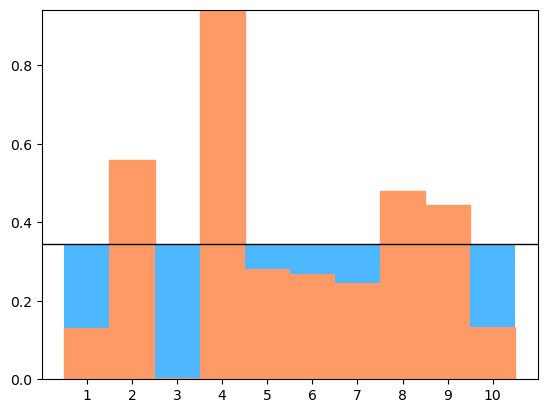
\includegraphics[scale = 0.6]{simple_water.png}
        \caption{visualization of water filling}
    \end{figure}
    \begin{figure}[H]
        \centering
        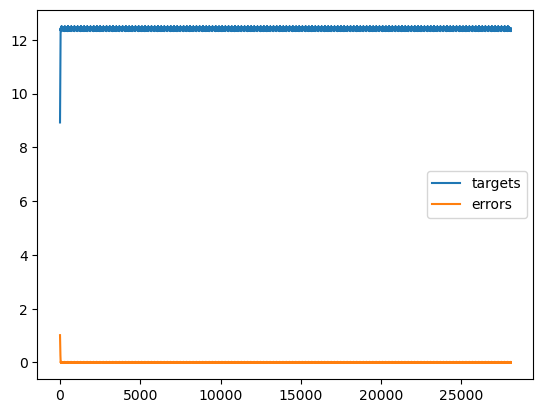
\includegraphics[scale = 0.6]{simple_te.png}
        \caption{targets and errors during iterations}
    \end{figure}
    \begin{figure}[H]
        \centering
        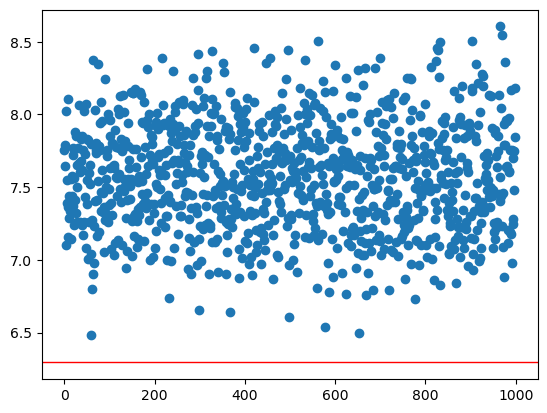
\includegraphics[scale = 0.6]{simple_random.png}
        \caption{compared with ``monkey"}
    \end{figure}
    \
    \newline
    \indent As you can see, in fig[2], the line seems to be quite wide, its because the x-label is to large and the target keeps vibrate even it comes to 25000 times iterations.
    
    To see it more clearly, I make it stop when iterations comes to 100, and the figure is as below:
    \begin{figure}[H]
        \centering
        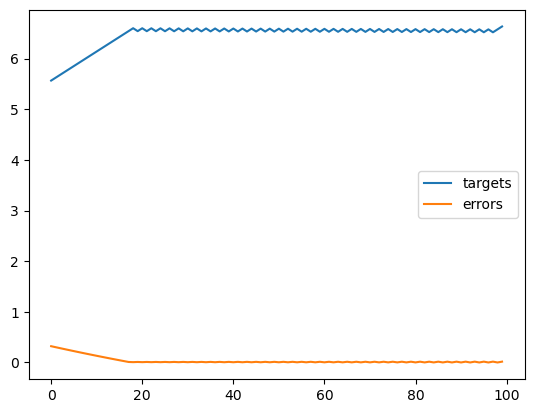
\includegraphics[scale = 0.75]{simple_te_100.png}
        \caption{targets and errors under 100 times iterations}
    \end{figure}

    This time, it's quite clear to see the vibration, and correspondingly\\
    $\sum_{i=1}^{n} x_i = 0.9834414024368723$, which can't achieve our precision.

    Therefore, the simple way can't achieve our standard, so let's turn to the descent method! 
    \subsection{the General Descent}
    \
    \newline
    \indent Here I provide the result of two independent experiments, and you can see, by using the General Descent, we can obtain an ideal result.

    And the detailed data for the experiment is:
    \begin{itemize}
        \item Experiment 1:
        \begin{itemize}
            \item $\sum_{i=1}^{n} x_i = 0.9999990075794267$
            \item $horizontal_line = 0.5364982106984345$
            \item $iterations = 1041$ 
        \end{itemize}
        \item Experiment 2:
        \begin{itemize}
            \item $\sum_{i=1}^{n} x_i = 1.0000009971989834$
            \item $horizontal_line = 0.3793815661631934$
            \item $iterations = 2143$
        \end{itemize}
    \end{itemize}
    \begin{figure}[H]
        \centering
        \subfigure[experiment 1]{
        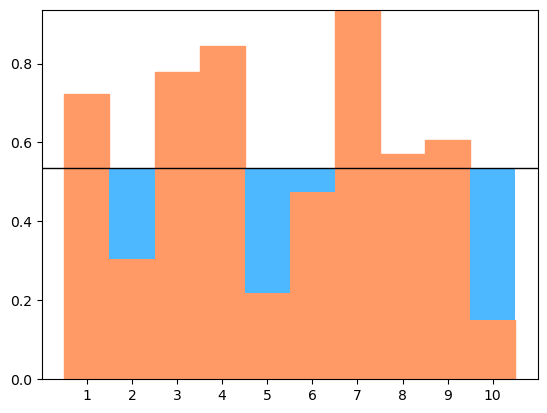
\includegraphics[scale=0.4]{gen_des_water.png}
        }
        \quad
        \subfigure[experiment 2]{
        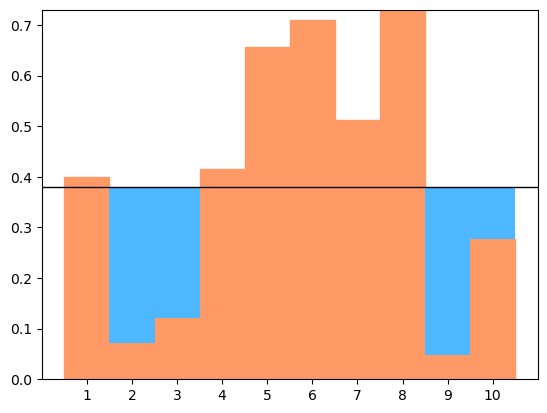
\includegraphics[scale=0.4]{gen_des_water2.png}
        }
        \caption{visualization of water filling}
    \end{figure}
    \begin{figure}[H]
        \centering
        \subfigure[experiment 1]{
        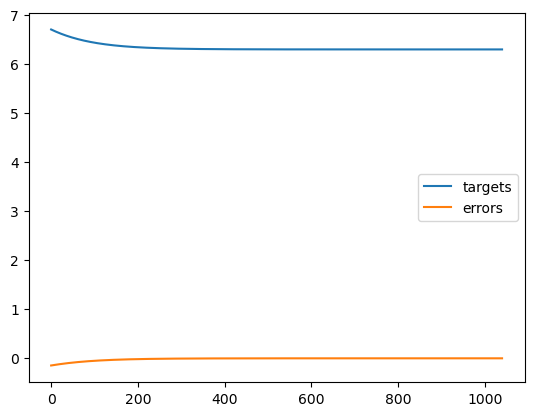
\includegraphics[scale=0.4]{gen_des_te.png}
        }
        \quad
        \subfigure[experiment 2]{
        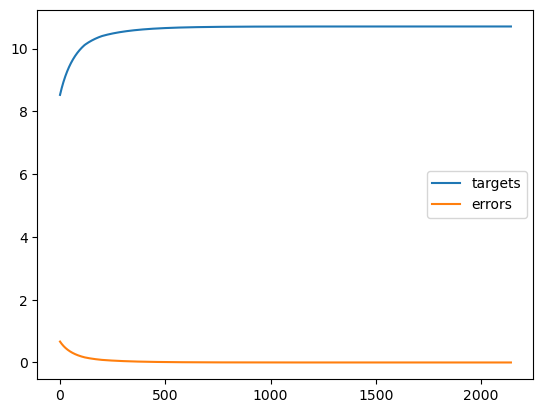
\includegraphics[scale=0.4]{gen_des_te2.png}
        }
        \caption{targets and errors during iterations}
    \end{figure}
    \begin{figure}[H]
        \centering
        \subfigure[experiment 1]{
        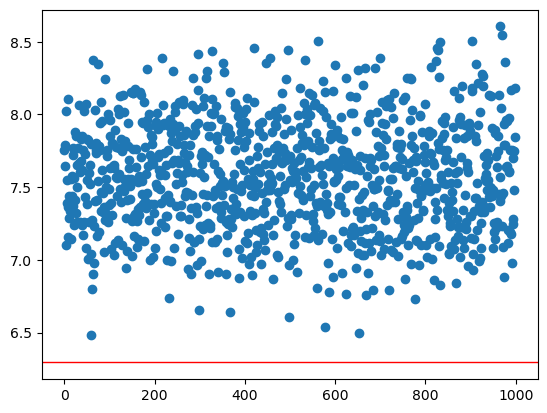
\includegraphics[scale=0.4]{gen_des_random.png}
        }
        \quad
        \subfigure[experiment 2]{
        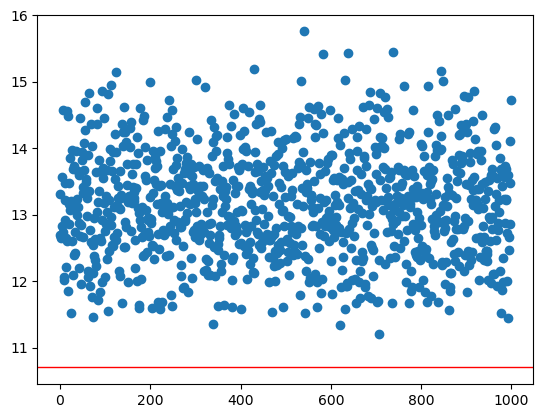
\includegraphics[scale=0.4]{gen_des_random2.png}
        }
        \caption{compared with ``monkey"}
    \end{figure}

    As you can see, in Figure 6, the graphic is very smooth under the elaborate adjust by error, and the vibration won't occur because the step\_size we choose can achieve approach in one direction.
    That is to say, using the way as $\nu += step\_size * error$ will not lead our solution after each iteration to the other side of final optimal solution.

    There's no doubt that it do does a good job!
    \subsection{the Gradient Descent}
    \
    \newline
    \indent At first, as I said in the Second Part, the Gradient Descent Method runs very slow, thus I change the precision to 0.01.

    And here is the data for it:
    \begin{itemize}
        \item $\sum_{i=1}^{n} x_i = 0.9995361774638688$, which only achieves precision of 0.001.
        \item $horizontal_line = 0.5948296449808184$
        \item $iterations = 12$
    \end{itemize}

    And the visualization graph is provided below:
    \begin{figure}[H]
        \centering
        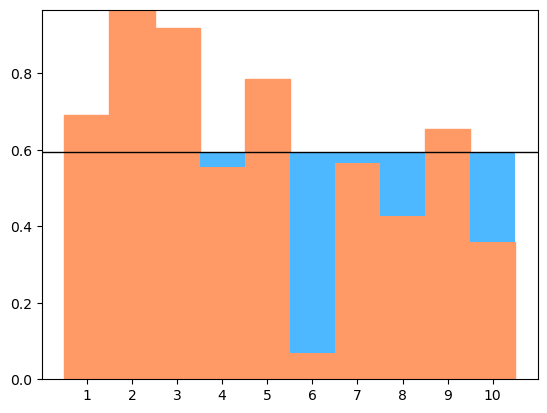
\includegraphics[scale = 0.8]{grad_des_water.png}
        \caption{visualization of water filling}
    \end{figure}
    \begin{figure}[H]
        \centering
        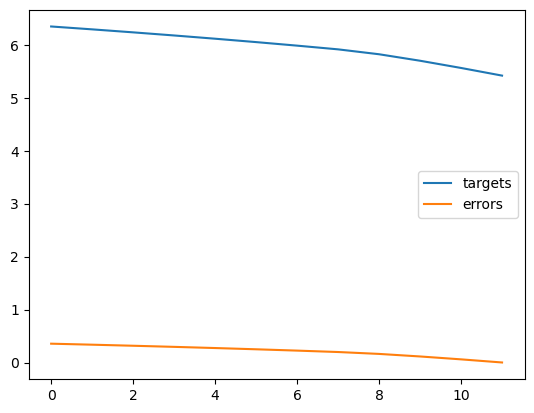
\includegraphics[scale = 0.8]{grad_des_te.png}
        \caption{targets and errors during iterations}
    \end{figure}
    \begin{figure}[H]
        \centering
        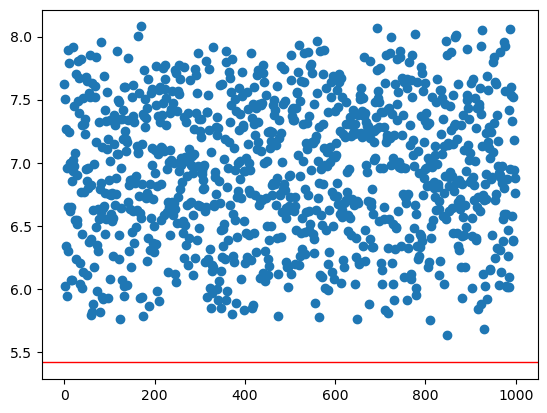
\includegraphics[scale = 0.8]{grad_des_random.png}
        \caption{compared with ``monkey"}
    \end{figure}

    As we can see, after 12 iterations, the algorithm has already had the ability to provide a result with very small bias. If we have enough time and sufficient computility, we can believe it will return a fantastic result even though the cost weighs a lot. So, it's not that perfect even though we might obtain a good result.
    \subsection{Bisection Method}
    \
    \newline
    \indent To conclude the above three algorithms, the result that the simple method returns are not that good, the Gradient Descent costs too much time and computility to achieve our goal (so do the Newton's Method whose results I don't show because I only get the result when the precision is 0.1, and $n=3$. And result with higher precision and more channels can't be obtained even though I have waited for nearly 10min).

    So, till now, under some comparison. We find it seems that only the optimized General Descent can efficiently return a good result. Here, fortunately, the Bisection Method also makes it! And it is even better for fewer iterations.

    And here is the result data, I also provide two seperate experiments:
    \begin{itemize}
        \item Experiment 1:
        \begin{itemize}
            \item $\sum_{i=1}^{n} x_i = 0.9999996766480913$
            \item $horizontal_line = 0.5474824842815678$
            \item $iterations = 22$ 
        \end{itemize}
        \item Experiment 2:
        \begin{itemize}
            \item $\sum_{i=1}^{n} x_i = 1.0000005952842315$
            \item $horizontal_line = 0.49176061581498987$
            \item $iterations = 21$
        \end{itemize}
    \end{itemize}

    And here are the corresponding visualized graph:
    \begin{figure}[H]
        \centering
        \subfigure[experiment 1]{
        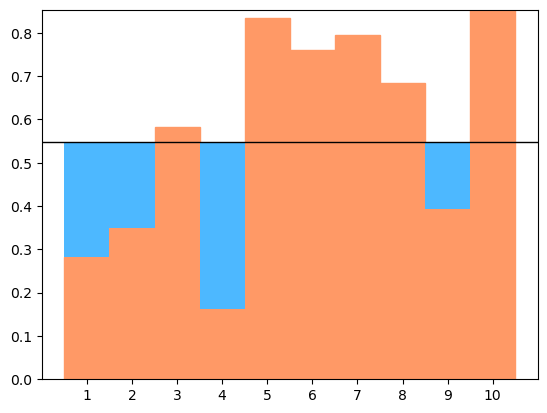
\includegraphics[scale=0.4]{bi_water.png}
        }
        \quad
        \subfigure[experiment 2]{
        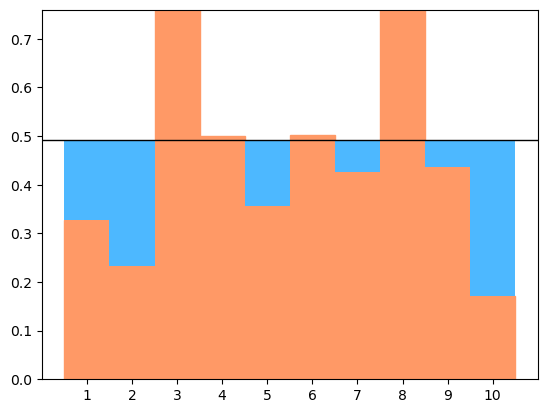
\includegraphics[scale=0.4]{bi_water2.png}
        }
        \caption{visualization of water filling}
    \end{figure}
    \begin{figure}[H]
        \centering
        \subfigure[experiment 1]{
        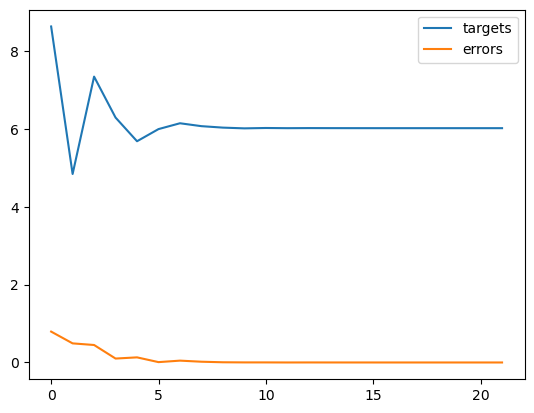
\includegraphics[scale=0.4]{bi_te.png}
        }
        \quad
        \subfigure[experiment 2]{
        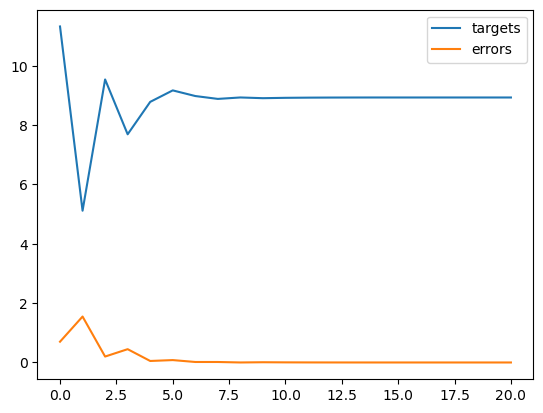
\includegraphics[scale=0.4]{bi_te2.png}
        }
        \caption{targets and errors during iterations}
    \end{figure}
    \begin{figure}[H]
        \centering
        \subfigure[experiment 1]{
        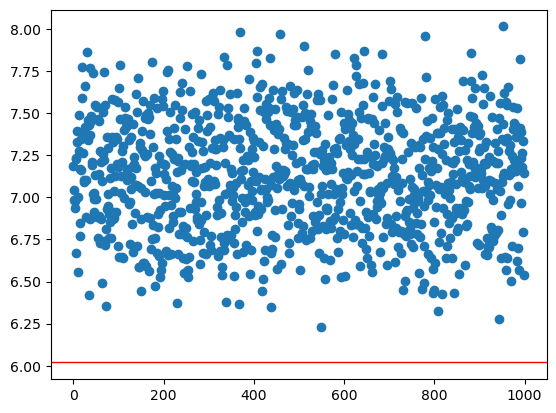
\includegraphics[scale=0.4]{bi_random.png}
        }
        \quad
        \subfigure[experiment 2]{
        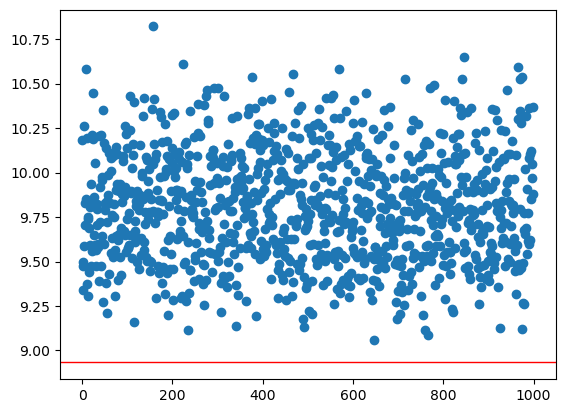
\includegraphics[scale=0.4]{bi_random2.png}
        }
        \caption{compared with ``monkey"}
    \end{figure}

    It should be explained that we can see the graphic vibrate severely at start, that is because when changing the $upper$ and $lower$ at begining, its value changes greatly because of the large value difference between $upper$ and $lower$ at start.
    
    We can see from both the data and the graph, the Bisection Method works perfect! And due to its much smaller iterations than the optimized General Descent, we can say it's the best among all the method I provide.
    
    \vspace*{1cm}
    \textbf{Done! Thanks for reading!}
\end{document}